\documentclass[11pt,a4paper]{scrartcl}

\usepackage{fontspec}
\usepackage{polyglossia}
\setdefaultlanguage{polish}

\usepackage[a4paper,margin=2.5cm]{geometry}
\usepackage[backend=biber,style=numeric,sorting=none]{biblatex}
\usepackage{graphicx}
\usepackage{float}
\usepackage{hyperref}
\usepackage{booktabs}
\usepackage{amsmath}
\usepackage{amssymb}
\usepackage{enumitem}
\usepackage{listings}
\usepackage{xcolor}

\addbibresource{bibliography.bib}

\hypersetup{
    colorlinks=true,
    linkcolor=black,
    citecolor=blue,
    urlcolor=blue
}

\subject{Metody Sztucznej Inteligencji 2 \textperiodcentered{} semestr letni 2025/26}
\title{Zastosowanie MCTS/UCT do gry Breakthrough 8$\times$8}
\subtitle{Raport końcowy}
\author{Hubert Sobociński \and Sebastian Rydz}
\date{\today}

\begin{document}

\maketitle

\begin{abstract}
% TODO: ~250 słów. Pokryj: cel projektu (zastosowanie MCTS/UCT do Breakthrough 6x6),
% metodę (4 warianty agenta + heurystyka), główne wyniki (H1-H4 wnioski),
% kluczowy wniosek (np. RAVE/PB efektywność, cross-over heurystyki, przewaga białych).
[STRESZCZENIE -- napisać po zakończeniu eksperymentów. Na bazie konspektu i wykresów.]
\end{abstract}


\newpage
\tableofcontents
\newpage

\section{Wstęp}
\label{sec:wstep}

\subsection{Gra Breakthrough}

\textbf{Breakthrough} to dwuosobowa gra strategiczna z pełną informacją,
wynaleziona przez Dana Troyka w 2000 roku (zwycięzca konkursu 8$\times$8 Game
Design Competition). Plansza jest kwadratowa, taka jak w szachach; każdy gracz
dysponuje pionkami ustawionymi w dwóch pierwszych rzędach po swojej stronie.
Ruch pionka odbywa się o jedno pole do przodu -- prosto lub po skosie. Ruch
prosty jest możliwy wyłącznie na puste pole; ruch po skosie może być wykonany
na pole puste lub zajęte przez pionek przeciwnika (bicie). Bicie prosto jest
niedozwolone, a pionki nie mogą się cofać.

Gra kończy się zwycięstwem gracza, który:
\begin{enumerate}[nosep]
    \item doprowadzi pionek do ostatniego rzędu przeciwnika,
    \item zbije wszystkie pionki przeciwnika,
    \item uniemożliwi przeciwnikowi wykonanie jakiegokolwiek legalnego ruchu.
\end{enumerate}
Remis nie jest możliwy.

\subsection{Dlaczego gra Breakthrough 8$\times$8}

Gra spełnia wszystkie wymagania projektu:
\begin{itemize}[nosep]
    \item \textbf{Dwuosobowa, z pełną informacją, deterministyczna} -- kluczowe
          właściwości dla metod MCTS/UCT.
    \item \textbf{Umiarkowany branching factor} -- w typowej pozycji na planszy
          8$\times$8 liczba legalnych ruchów wynosi 15--30. Głębokość partii to
          40--80 ruchów.
    \item \textbf{Proste zasady, ale trudna strategicznie} -- mimo prostych
          zasad wymaga planowania na wiele ruchów naprzód (tworzenie łańcuchów
          pionków, kontrola kolumn, poświęcenia pionka w celu wygranej).
    \item \textbf{Niszowa} -- w odróżnieniu od szachów czy warcabów gra nie jest
          aż tak popularna.
    \item \textbf{Wariant 8$\times$8 nie został rozwiązany} -- Saffidine i in.\
          \cite{saffidine2011solving} rozwiązali warianty do planszy 6$\times$5,
          a Björnsson i in.\ \cite{bjornsson2026solving} rozwiązali planszę
          6$\times$6 (w obu przypadkach wygrywa pierwszy gracz). Klasyczna
          plansza 8$\times$8 pozostaje otwarta, co zostawia miejsce na
          eksperymenty porównawcze bez znanego ,,perfekcyjnego gracza''.
\end{itemize}

\subsection{Cel projektu}

Celem projektu jest zaprojektowanie i implementacja agentów grających
w Breakthrough 8$\times$8 z wykorzystaniem algorytmu Monte Carlo Tree Search
w wariancie UCT oraz jego rozszerzeń, a następnie eksperymentalne porównanie
ich skuteczności.

W szczególności projekt obejmuje:
\begin{itemize}[nosep]
    \item implementację bazowego algorytmu UCT,
    \item implementację dwóch rozszerzeń UCT:
          \begin{itemize}[nosep]
              \item RAVE (z literatury),
              \item Progressive Bias (z literatury),
          \end{itemize}
    \item implementację gracza heurystycznego (minimax alfa-beta),
    \item porównanie jakości gry powyższych podejść,
    \item stworzenie interfejsu człowiek--komputer i przeprowadzenie testów
          z użytkownikami.
\end{itemize}

\subsection{Hipotezy badawcze}

W projekcie weryfikujemy sześć hipotez:

\begin{itemize}
    \item[\textbf{H1}] \textbf{RAVE poprawia skuteczność względem bazowego UCT.}
          Agent UCT rozszerzony o RAVE osiąga istotnie wyższy win-rate niż czysty
          UCT przy tym samym budżecie iteracji.

    \item[\textbf{H2}] \textbf{Progressive Bias poprawia skuteczność względem
          bazowego UCT.} Agent UCT z Progressive Bias osiąga istotnie wyższy
          win-rate niż czysty UCT, szczególnie przy niskich budżetach iteracji.

    \item[\textbf{H3}] \textbf{Heurystyka specjalistyczna przewyższa MCTS przy
          małym budżecie iteracji, jednak przegrywa przy wysokim.} Agent minimax
          alfa-beta z heurystyką domenową wygrywa z UCT przy małych budżetach
          iteracji, ale przegrywa przy dużych.

    \item[\textbf{H4}] \textbf{Przewaga pierwszego gracza.} W Breakthrough
          pierwszy gracz ma niewielką przewagę -- podobna sytuacja jak
          w szachach.

    \item[\textbf{H5}] \textbf{Stała eksploracji $c$ w UCT ma nieliniowy wpływ
          na siłę gry.} Istnieje optymalna wartość $c^\star$ maksymalizująca
          win-rate agenta UCT w Breakthrough 8$\times$8. Zarówno zbyt niska
          (nadmierna eksploatacja), jak i zbyt wysoka (nadmierna eksploracja)
          wartość $c$ prowadzi do istotnego spadku skuteczności.

    \item[\textbf{H6}] \textbf{Czas podejmowania decyzji MCTS rośnie w środkowej
          fazie gry.} Przy stałym budżecie iteracji średni czas na ruch agenta
          MCTS jest najwyższy w fazie środkowej partii (ruchy 15--40), gdy
          branching factor jest największy, i maleje w otwarciu oraz końcówce.
\end{itemize}


\section{Przegląd literatury}
\label{sec:literatura}

W niniejszej sekcji przedstawiamy genezę algorytmu Monte Carlo Tree Search,
najważniejsze rozszerzenia istotne dla tego projektu oraz literaturę
dotyczącą gry Breakthrough w kontekście MCTS.

\subsection{Geneza MCTS i UCT}

Metoda Monte Carlo Tree Search została zaproponowana przez Coulom\,a
\cite{coulom2006efficient} jako algorytm przeszukiwania dla gry Go,
gdzie wcześniejsze podejścia oparte na alpha-beta nie potrafiły poradzić
sobie z dużym branching factor (typowo 200--400 ruchów w pozycji).
Kluczowa innowacja Coulom\,a: zamiast przeszukiwać drzewo gry do pełnej
głębokości i ewaluować liście funkcją heurystyczną, rozwijano drzewo
selektywnie i zamiast ewaluacji symulowano losowe partie do końca,
agregując wyniki w statystykach Monte Carlo per stan.

W tym samym roku Kocsis i Szepesvári~\cite{kocsis2006bandit} wprowadzili
algorytm UCT (Upper Confidence Bounds applied to Trees), łączący metodę
Coulom\,a z regułą wyboru z teorii bandytów wieloramiennych. Funkcja
selekcji UCB1 daje matematycznie ugruntowany kompromis między
eksploatacją węzłów już dobrze zbadanych a eksploracją mniej odwiedzonych.

Kompleksowy przegląd MCTS i jego wariantów do roku 2012 przedstawili
Browne et al.~\cite{browne2012survey} ze szczególnym uwzględnieniem
zastosowań poza Go: gry kart, gry planszowe, planowanie. Praca ta jest
podstawowym punktem odniesienia metodologicznego dla niniejszego projektu.

\subsection{Rozszerzenia MCTS istotne dla projektu}

\paragraph{RAVE (Rapid Action Value Estimation).}
Gelly i Silver~\cite{gelly2011monte} wprowadzili technikę RAVE oraz
powiązane statystyki AMAF (All-Moves-As-First), będące rozszerzeniem
wcześniejszych prac nad polityką uczenia w grze Go. Główna idea: jeśli
ruch $m$ okazywał się dobry w rolloutach wychodzących z poddrzewa węzła
$n$, to $m$ jest również prawdopodobnie dobry z samego $n$, nawet jeśli
$m$ nie był jeszcze próbowany jako pierwszy. Selekcja RAVE blenduje
oszacowania UCT i AMAF z wagą $\beta$ malejącą wraz z liczbą odwiedzin
węzła --- oryginalna formuła $\beta(n, \tilde{n})$ uwzględnia zarówno
liczbę odwiedzin węzła $n$, jak i liczbę odwiedzin AMAF $\tilde{n}$.

W~grze Go RAVE daje silne przyspieszenie zbieżności --- Gelly i Silver
raportują 20--40\% wzrost win-rate przy tym samym budżecie iteracji.
Kluczowe założenie sukcesu: \emph{translation invariance} wartości ruchu ---
postawienie kamienia w punkcie $(x, y)$ ma podobną wartość w różnych
kontekstach taktycznych.

\paragraph{Progressive Bias / Progressive Strategies.}
Chaslot et al.~\cite{chaslot2008progressive} zaproponowali rodzinę
,,progressive strategies'' wstrzykujących wiedzę domenową do MCTS.
Centralna z technik --- Progressive Bias --- dodaje do funkcji selekcji
człon $H(m) / (n + 1)$, gdzie $H(m)$ jest oszacowaniem heurystycznym
ruchu $m$. Człon ten dominuje wczesne iteracje (gdy $n$ jest małe),
po czym zanika z rosnącym $n$, oddając kontrolę statystykom UCB1.
Chaslot pokazał, że taka kombinacja przewyższa zarówno czyste UCT,
jak i czystą heurystykę, w grze Go i innych domenach.

\paragraph{MAST (Move-Average Sampling Technique).}
Finnsson i Björnsson~\cite{finnsson2008simulation} w kontekście General Game
Playing zaproponowali MAST --- globalną tabelę średnich wyników per ruch,
aktualizowaną po każdej symulacji. Ta tabela następnie wpływa na rolloutsy
(softmax/$\epsilon$-greedy zamiast uniform random). MAST był rozważany
jako alternatywna druga modyfikacja UCT (zamiast Progressive Bias),
ostatecznie odrzucony jako mniej spójny tematycznie z heurystyką H3.

\paragraph{Pozostałe rozszerzenia.}
Lorentz~\cite{lorentz2016early} opisuje \emph{Early Playout Termination}:
wczesne kończenie symulacji w stanach o oczywistym zwycięzcy, znacząco
przyspieszające MCTS w grach z wyraźną strukturą terminalu (jak Breakthrough).
Inne rozszerzenia warte uwagi (poza zakresem tego projektu): UCT z transposition
tables, virtual loss dla zrównoleglenia, decisive/anti-decisive moves
(Teytaud \& Teytaud, AAAI 2010).

\subsection{Breakthrough w literaturze MCTS}

\paragraph{Status rozwiązaniowy gry.}
Saffidine et al.~\cite{saffidine2011solving} opracowali techniki ,,race
patterns'' i Job-Level Proof Number Search, pozwalające im rozwiązać
warianty Breakthrough do planszy 6$\times$5 włącznie; we wszystkich
\emph{wygrywa pierwszy gracz}. Niedawno Björnsson et al.~\cite{bjornsson2026solving}
rozwiązali również planszę 6$\times$6 (także na korzyść pierwszego gracza).
Klasyczna plansza 8$\times$8 pozostaje natomiast nierozwiązana --- nie ma
znanego solwera o ograniczonych zasobach pamięciowych zdolnego do pełnego
przeszukania jej drzewa. To czyni Breakthrough 8$\times$8 atrakcyjnym
benchmarkiem: nie istnieje wyrocznia ,,perfekcyjnego gracza'' definiująca
sufit jakości, więc porównanie wariantów MCTS ma realną wartość badawczą.

\paragraph{Heurystyki ewaluacji.}
Lorentz~\cite{lorentz2011breakthrough} (w pracy nad EinStein würfelt nicht!,
ale stosowanej również do Breakthrough) opisuje proste heurystyki ewaluacji
pozycji zawierające zaawansowanie pionków, materiał oraz bezpieczeństwo
struktury (pionki na krawędziach są bezpieczniejsze, ponieważ mogą zostać
zbite tylko z jednej strony zamiast dwóch). Te elementy stanowią podstawę
naszej implementacji \texttt{HeuristicAgent}.

\paragraph{Branching factor i głębokość.}
W typowej pozycji Breakthrough 8$\times$8 liczba legalnych ruchów wynosi
około 15--30, a głębokość partii (przy losowej grze) to 40--80 półruchów.
Z naszych eksperymentów (sekcja~\ref{sec:wyniki}) średnia długość partii
UCT vs UCT na planszy 8$\times$8 wynosi ok.\ 57 ruchów. Branching factor
zalicza Breakthrough do gier ,,małych'' z punktu widzenia MCTS ---
znacznie mniej niż Go (200--400), porównywalnie do Hex (odpowiadający
rozmiar $11 \times 11$ ma branching ok. 80--100).

\paragraph{Status badawczy Breakthrough 8$\times$8.}
Klasyczna plansza 8$\times$8 pozostaje \emph{nierozwiązana} --- mimo postępów
w rozwiązywaniu mniejszych wariantów (do 6$\times$5 \cite{saffidine2011solving}
oraz 6$\times$6 \cite{bjornsson2026solving}), dla 8$\times$8 nie istnieje znany
,,perfekcyjny gracz''. Brak odniesienia do optimum czyni z 8$\times$8
wdzięczny poligon dla \emph{porównawczych} badań empirycznych nad wariantami
MCTS, gdzie miarą jest względna siła agentów, a nie odległość od gry idealnej.

\section{Metoda}
\label{sec:metoda}

W tej sekcji opisujemy szczegóły algorytmiczne i implementacyjne wszystkich
agentów porównywanych w eksperymentach.

\subsection{Reprezentacja stanu gry}

Stan gry Breakthrough w naszej implementacji jest reprezentowany przez parę
bitboardów $u_{64}$: jeden dla pionków białych, jeden dla czarnych. Bit $i$
odpowiada polu $i = r \cdot c + k$, gdzie $r$ to numer rzędu (0-indeksowany
od dołu), $k$ to numer kolumny, a $c$ to liczba kolumn planszy. Dla planszy
6$\times$6 wszystkie 36 pól mieszczą się w jednym \texttt{u64}, dla 8$\times$8
zajmujemy całe 64 bity. Stan gry zawiera również:
flagę \texttt{white\_to\_move};
licznik \texttt{move\_count};
wartość hash Zobrist $\in \{0, \ldots, 2^{64}-1\}$ zaktualizowaną przyrostowo;
stałe maski (lewa i prawa krawędź, plansza, rzędy zwycięskie).

\paragraph{Generowanie ruchów.}
Korzystamy z operacji bitowych z maskowaniem krawędzi przed przesunięciem,
co eliminuje błąd ,,wraparound''. Dla białego (porusza się ku wyższym wierszom):
\begin{align*}
\text{prosto} &= (W \ll c) \,\&\, \text{empty} \,\&\, \text{board\_mask} \\
\text{ukos lewy} &= ((W \,\&\, \overline{\text{left\_edge}}) \ll (c-1)) \,\&\, (\text{empty} \cup B) \,\&\, \text{board\_mask} \\
\text{ukos prawy} &= ((W \,\&\, \overline{\text{right\_edge}}) \ll (c+1)) \,\&\, (\text{empty} \cup B) \,\&\, \text{board\_mask}
\end{align*}
gdzie $W$, $B$ to bitboardy białych i czarnych, $\overline{X}$ to negacja.
Dla czarnego (przesunięcia w dół) ruchy są symetryczne, używają operatora $\gg$.

\paragraph{Detekcja końca gry.}
Cztery warunki sprawdzane w kolejności (od najtańszego do najdroższego):
(1) biały dotarł do ostatniego rzędu;
(2) czarny dotarł do rzędu 0;
(3) jeden z graczy stracił wszystkie pionki;
(4) gracz na ruchu nie ma legalnych ruchów (przegrywa).

\paragraph{Hash Zobrist.}
Tablica losowych $u_{64}$ rozmiar $2 \cdot \text{rows} \cdot \text{cols}$
generowana raz, deterministycznie seedowana. Hash stanu = XOR wartości tablicy
dla każdego pionka na planszy. Współdzielona przez referencję
(\texttt{Arc<Vec<u64>>}) między wszystkimi instancjami stanu, dzięki czemu klonowanie
\texttt{GameState} jest stałoczasowe.

\paragraph{Walidacja krzyżowa.}
Dla pewności poprawności silnika, równolegle z implementacją w Ruście została
napisana referencyjna implementacja w czystym Pythonie (priorytet czytelności).
Test \texttt{test\_rust\_vs\_python.py} gra 1000 losowych partii i porównuje
po każdym ruchu zbiory legalnych ruchów, stan terminalny, zwycięzcę i
reprezentację tekstową. Pełna zgodność jest warunkiem koniecznym przed
uruchomieniem eksperymentów.

\subsection{Vanilla UCT (Kocsis \& Szepesvári 2006)}

Klasyczny algorytm 4-fazowego MCTS \cite{kocsis2006bandit}:

\begin{enumerate}[nosep]
    \item \textbf{Selekcja.} Począwszy od korzenia, w każdym wewnętrznym węźle
          $s$ wybieramy potomka maksymalizującego UCB1:
          \begin{equation}
              \text{score}(c) = \frac{\text{wins}(c)}{\text{visits}(c)}
                              + c_{\text{exp}} \sqrt{\frac{\ln \text{visits}(s)}{\text{visits}(c)}}
              \label{eq:ucb1}
          \end{equation}
          Dla potomka z $\text{visits} = 0$ zwracamy $\infty$ (forsujemy
          jego eksplorację).
    \item \textbf{Ekspansja.} W węźle z nierozwiniętymi ruchami wybieramy
          jeden losowy nierozwinięty ruch i tworzymy nowy węzeł potomny.
    \item \textbf{Symulacja.} Od nowego węzła gramy losowo (uniform) do
          terminala.
    \item \textbf{Backpropagation.} Wynik symulacji przekazywany jest
          w górę drzewa; na każdym węźle aktualizujemy:
          $\text{visits}(n) \mathrel{{+}{=}} 1$, oraz
          $\text{wins}(n) \mathrel{{+}{=}} 1$ jeśli wygrał gracz, który zagrał
          ruch \emph{do} tego węzła.
\end{enumerate}

\paragraph{Konwencja perspektywy.}
$\text{wins}(c)$ liczone jest z perspektywy gracza, który wykonał ruch $c$
(czyli gracza znajdującego się na ruchu w rodzicu $c$). Ta konwencja
zapewnia, że UCB1 w wzorze (\ref{eq:ucb1}) wybiera ruch dający
maksymalne wygrane dla gracza wybierającego --- dokładnie to, czego oczekujemy
od minimax-spójnej selekcji.

\paragraph{Implementacja.}
Pula węzłów to płaska \texttt{Vec<UctNode>} indeksowana \texttt{usize}
zamiast wskaźników. Węzły nie przechowują pełnego \texttt{GameState} (oszczędność
pamięci); stan przy schodzeniu od korzenia jest rekonstruowany przez
ponowne aplikowanie ruchów. Cena: $O(\text{depth})$ klonowań stanu na
iterację (akceptowalne ze względu na taniość klonowania $\sim$80B + Arc).

Eksponowany do Pythona przez PyO3 jako \texttt{UctAgent(iterations, c, seed)}.

\subsection{UCT + RAVE (Gelly \& Silver 2011)}

\paragraph{Algorytm.}
Każdy węzeł $s$ przechowuje, oprócz statystyk UCT, dodatkowe statystyki AMAF
(All-Moves-As-First): mapę kluczowaną kodem ruchu \texttt{from*64 + to},
zawierającą liczbę odwiedzin $\tilde{n}(s, a)$ i wygranych $\tilde{w}(s, a)$
dla ruchu $a$ jako pierwszego z $s$.

W fazie selekcji potomek $c$ rodzica $s$ jest oceniany formułą zmieszaną
\cite{gelly2011monte}:
\begin{align}
    \text{score}(c) &= (1 - \beta) Q_{\text{UCT}}(c) + \beta Q_{\text{RAVE}}(c) + c_{\text{exp}} \sqrt{\frac{\ln N(s)}{n(c)}} \label{eq:rave}\\
    \beta(n, \tilde{n}) &= \frac{\tilde{n}}{n + \tilde{n} + 4 n \tilde{n} b^2} \label{eq:beta}
\end{align}
gdzie $Q_{\text{UCT}}(c) = \text{wins}(c) / \text{visits}(c)$ to ocena UCT,
$Q_{\text{RAVE}}(c) = \tilde{w}(s, a_c) / \tilde{n}(s, a_c)$ to wartość AMAF
ruchu $a_c$ wiodącego do $c$ (zapisana w $s$, indeksowana kodem ruchu),
$b^2$ to hiperparametr formuły Silvera (\ref{eq:beta}).

\paragraph{Aktualizacja AMAF w backpropagation.}
Dla każdego węzła $n$ na ścieżce od korzenia do liścia: niech $p_n$ oznacza
gracza na ruchu w $n$. Dla każdego ruchu $m$ zagranego w fazie in-tree
\emph{poniżej} $n$ \emph{lub} w fazie symulacji, jeśli ruch wykonał gracz
$p_n$:
\begin{itemize}[nosep]
    \item $\tilde{n}(n, m) \mathrel{{+}{=}} 1$,
    \item $\tilde{w}(n, m) \mathrel{{+}{=}} 1$, jeśli $p_n$ wygrał symulację.
\end{itemize}

Włączenie ruchów in-tree (a nie tylko symulacyjnych) jest kluczowe ---
pierwsza wersja implementacji pomijała te ruchy, prowadząc do drastycznej
porażki RAVE w eksperymentach (patrz~sekcja~\ref{sec:llm}).

\paragraph{Wybór hiperparametru $b^2$.}
Klasyczna wartość Silvera ($b^2 = 10^{-4}$) okazała się nieoptymalna
dla Breakthrough --- daje $\beta$ tak bliskie 1, że Q-RAVE dominuje selekcję.
Po zamiataniu (sweep) $b^2 \in \{10^{-6}, \ldots, 10^{-1}\}$, wybraliśmy
$b^2 = 10^{-2}$ jako najlepiej działającą wartość.

Eksponowany jako \texttt{RaveAgent(iterations, c, rave\_k, seed)},
gdzie \texttt{rave\_k} dla zachowania kompatybilności API jest interpretowane
jako $b^2$.

\subsection{UCT + Progressive Bias (Chaslot et al. 2008)}

\paragraph{Algorytm.}
Selekcja potomka rozszerza UCB1 o człon biasu malejący z liczbą odwiedzin
\cite{chaslot2008progressive}:
\begin{equation}
    \text{score}(c) = Q_{\text{UCT}}(c) + c_{\text{exp}} \sqrt{\frac{\ln N(s)}{n(c)}} + w_{\text{bias}} \cdot \frac{H(c)}{n(c) + 1}
\end{equation}
gdzie $H(c) \in [0, 1]$ jest wartością heurystyki ruchu wiodącego do $c$,
a $w_{\text{bias}}$ to waga biasu (= 1.0 w naszych eksperymentach).
Człon $1/(n(c)+1)$ powoduje naturalny zanik biasu wraz ze wzrostem
liczby symulacji --- przy rosnącej $n(c)$ statystyki Q-UCT przejmują
sterowanie selekcją.

\paragraph{Funkcja heurystyczna $H$.}
Dla ruchu z pola $f$ na pole $t$ przy graczu $p$:
\begin{equation}
H(c) = \min\!\left(1{,}0, \quad \text{adv}(t, p) + b_{\text{cap}} \cdot [\text{ruch jest biciem}]\right)
\end{equation}
gdzie $\text{adv}(t, p) = t_{\text{row}} / (R-1)$ dla białego i $(R-1-t_{\text{row}}) / (R-1)$
dla czarnego (zaawansowanie pionka znormalizowane do $[0, 1]$ względem rzędu
docelowego), a $b_{\text{cap}} = 0{,}2$ to bonus za bicie. $R$ to liczba
rzędów planszy.

Eksponowany jako \texttt{ProgressiveBiasAgent(iterations, c, bias\_weight, seed)}.

\subsection{Heurystyczny gracz alpha-beta}

\paragraph{Funkcja ewaluacji.}
$f: \text{State} \times \text{Player} \to \mathbb{R}$, dodatnia gdy korzystna
dla \emph{Player}:
\begin{equation}
f(s, p) = \pm \left( w_{\text{adv}} \cdot \Delta_{\text{advancement}} + w_{\text{mat}} \cdot \Delta_{\text{material}} + w_{\text{mob}} \cdot \Delta_{\text{mobility}} \right)
\end{equation}
gdzie:
\begin{itemize}[nosep]
    \item $\Delta_{\text{advancement}} = \sum_{\text{pionków białych}} \frac{r}{R-1} - \sum_{\text{pionków czarnych}} \frac{R-1-r}{R-1}$ ---
          różnica zaawansowania pionków (znormalizowana do rzędu),
    \item $\Delta_{\text{material}}$ = liczba pionków białych $-$ liczba pionków czarnych,
    \item $\Delta_{\text{mobility}} = |\text{legalne ruchy}|$ z znakiem (+ jeśli na ruchu jest biały, $-$ wpp).
\end{itemize}
Wagi: $w_{\text{adv}} = 1{,}0$, $w_{\text{mat}} = 3{,}0$, $w_{\text{mob}} = 0{,}1$
(dobrane na podstawie szacunków z literatury \cite{lorentz2011breakthrough}
i kalibracji wstępnej). Dla terminala: $\pm 1000$ (wartość dominująca pozostałe składniki).

\paragraph{Przeszukiwanie alpha-beta.}
Klasyczny negamax z odcięciem $\alpha\beta$, głębokość 5 półruchów.
Brak heurystyk porządkujących ruchy (move ordering) --- niepotrzebne
dla 6$\times$6 (depth 5 zajmuje $\sim$30 ms).

Eksponowany jako \texttt{HeuristicAgent(depth=5, weights=None)}.

\subsection{Architektura implementacji}

\paragraph{Stos technologiczny.}
Rdzeń obliczeniowy (silnik gry, wszystkie agenci, ewaluacja) zaimplementowany
w języku Rust. Orchestracja eksperymentów, GUI i analiza wyników w Pythonie 3.12.
Wiązanie Rust $\leftrightarrow$ Python przez PyO3 0.22 z budowaniem przez maturin.

\paragraph{Struktura repozytorium.}
\begin{verbatim}
breakthrough-mcts/
  src/                              # Rust
    game.rs                         # Bitboard GameState
    mcts/{uct,rave,progressive_bias}.rs
    heuristic.rs                    # alpha-beta
  python/breakthrough/
    reference_game.py               # Walidacja krzyżowa
    gui.py                          # Pygame GUI
    experiments/                    # Run_h{1,2,3,4}.py
  tests/test_rust_vs_python.py      # Walidacja silnika
  notebooks/                        # Skrypty analityczne
  report/                           # Niniejszy dokument
\end{verbatim}

\paragraph{Reprodukowalność.}
Generator: Xoshiro256++ \cite{vigna2017}. Master seed wyprowadza
deterministycznie seedy partii (SHA-256). Każda partia ma jawnie zapisany seed
w logu JSONL --- możliwa pełna replikacja pojedynczej partii.

\paragraph{Decyzja o zrównolegleniu.}
\textbf{MCTS jest sekwencyjny}, zrównoleglenie odbywa się wyłącznie na poziomie
batchowania eksperymentów (\texttt{ProcessPoolExecutor}). Decyzja motywowana
czystością metodologiczną porównań --- porównujemy algorytmy, nie zrównoleglenie.
Tree parallelization (virtual loss) ani root parallelization \emph{nie} są
zaimplementowane.

\section{Plan eksperymentów}

% TODO: Opis 4 eksperymentów (H1-H4) + metodologia. Pokryj:
%  - H1: RAVE vs UCT, budżety {1k, 5k, 10k}
%  - H2: Progressive Bias vs UCT, ten sam zakres
%  - H3: Heurystyka (alpha-beta d=5) vs UCT przy budżetach {200, 500, 1k, 5k, 10k}
%  - H4: UCT vs UCT (same agent both sides), board sizes 6x6, 6x8, 8x8
%  - Liczba partii: 60 na parę (30 na każdą stronę), H4: 100
%  - Reprodukowalność: master seed -> per-game seed via SHA256
%  - Statystyka: Wilson 95% CI dla win rate

\subsection{H1: RAVE vs UCT}
[Konfiguracja, oczekiwania.]

\subsection{H2: Progressive Bias vs UCT}
[Konfiguracja, oczekiwania.]

\subsection{H3: Heurystyka vs MCTS}
[Konfiguracja, oczekiwania na cross-over.]

\subsection{H4: Przewaga pierwszego gracza}
[Konfiguracja, oczekiwania.]

\subsection{Metodologia statystyczna}
[Wilson CI, liczba partii, reprodukowalność.]

\section{Wyniki}
\label{sec:wyniki}

W niniejszej sekcji prezentujemy wyniki sześciu eksperymentów odpowiadających
hipotezom H1--H6, wszystkie przeprowadzone na klasycznej planszy 8$\times$8.
Wszystkie odsetki wygranych raportowane są wraz z 95\%
przedziałami ufności wyliczanymi metodą Wilsona \cite{wilson1927probable}.

\subsection{H1: RAVE vs vanilla UCT}
\label{sec:wyniki-h1}

\begin{figure}[ht]
    \centering
    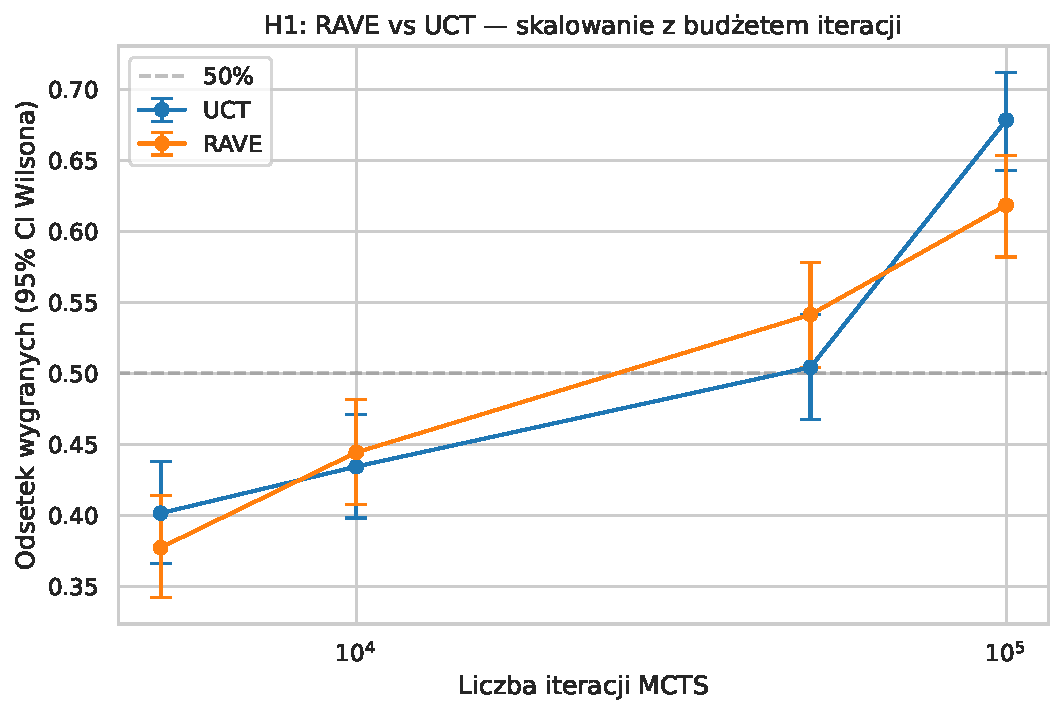
\includegraphics[width=0.85\textwidth]{figures/h1_rave_vs_uct}
    \caption{Skalowanie odsetków wygranych RAVE i UCT z budżetem iteracji
    (8$\times$8, turniej round-robin). Punkty pokazują ogólny win-rate każdego
    agenta we wszystkich rozegranych przez niego partiach, słupki błędów to
    95\% CI Wilsona. Linia 50\% oznacza neutralność. Obie metody zyskują z budżetem;
    RAVE nie wyprzedza UCT przy żadnym budżecie.}
    \label{fig:h1}
\end{figure}

\paragraph{Dane liczbowe --- bezpośrednie mecze RAVE vs UCT przy tym samym
budżecie (n=100 partii na budżet):}
\begin{center}
\begin{tabular}{rcccc}
\toprule
\textbf{Budżet} & \textbf{RAVE wygrywa} & \textbf{Win-rate} & \textbf{$p$ (vs 0,5)} & \textbf{Status} \\
\midrule
5\,000   & 49/100 & 49,0\% & 0,92 & parytet \\
10\,000  & 48/100 & 48,0\% & 0,76 & parytet \\
50\,000  & 54/100 & 54,0\% & 0,48 & parytet \\
100\,000 & 39/100 & \textbf{39,0\%} & 0,035 & RAVE gorszy \\
\bottomrule
\end{tabular}
\end{center}

Hipoteza H1 jest \emph{sfalsyfikowana}: RAVE nie wygrywa istotnie z vanilla UCT
przy żadnym budżecie, a przy 100\,000 iteracji \emph{przegrywa} istotnie
statystycznie (39,0\%, $p = 0{,}035$). Rezultat jest odmienny od oczekiwań
literaturowych z dziedziny Go, gdzie RAVE przewyższa vanilla UCT przy każdym
praktycznym budżecie \cite{gelly2011monte}.

Interpretujemy to następująco: RAVE akumuluje wartości AMAF przez wszystkie
pozycje w drzewie i symulacjach, zakładając przesuwalność wartości ruchu
(translation invariance). Założenie to zachodzi w Go (kamień postawiony
w punkcie $X$ ma podobną wartość w różnych kontekstach), ale załamuje się
w Breakthrough, gdzie wartość ruchu (np.\ ,,pionek z pola $X$ na $Y$'') silnie
zależy od reszty pozycji. Sygnał AMAF jest więc niemal nieinformatywny;
przy największym budżecie staje się wręcz szkodliwy, podczas gdy vanilla UCT
efektywnie wykorzystuje rosnący budżet do precyzowania szacunków per-stan.
Zauważmy, że poprawność samej implementacji RAVE potwierdziliśmy niezależnie
(sekcja~\ref{sec:llm}): przy zneutralizowanym członie AMAF ($\beta \to 0$)
RAVE odtwarza siłę UCT, co dowodzi, że obserwowany spadek pochodzi z heurystyki
AMAF, a nie z błędu w szkielecie algorytmu.

\subsection{H2: Progressive Bias vs vanilla UCT}
\label{sec:wyniki-h2}

\begin{figure}[ht]
    \centering
    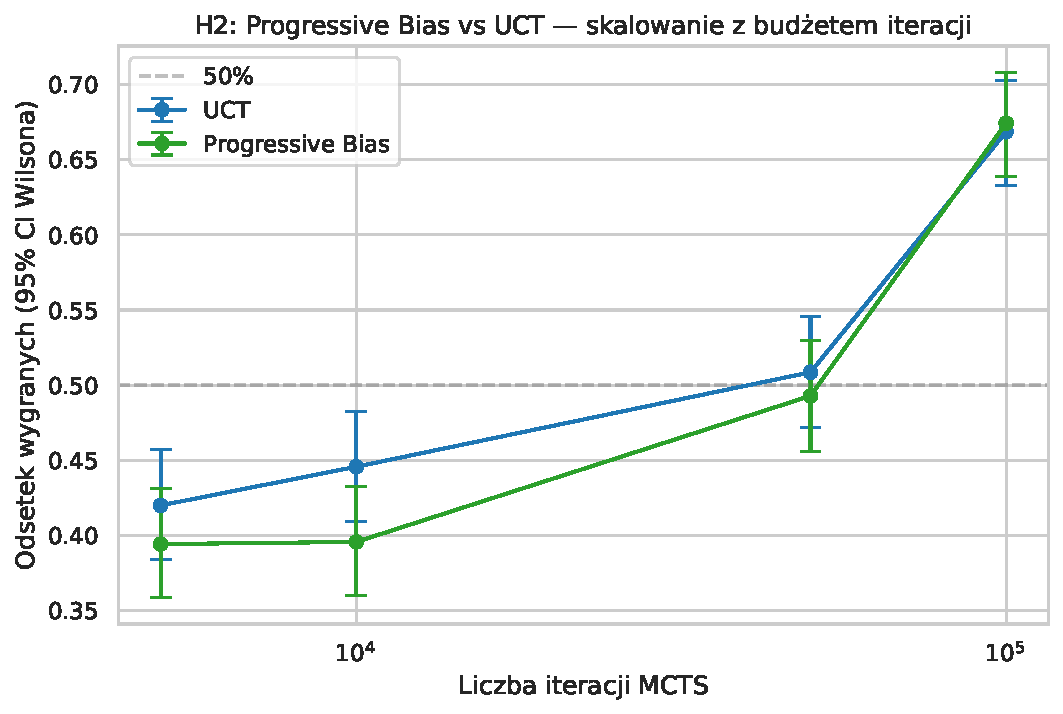
\includegraphics[width=0.85\textwidth]{figures/h2_pb_vs_uct}
    \caption{Skalowanie odsetków wygranych Progressive Bias i UCT (8$\times$8).
    Człon bias w selekcji oparty na heurystyce porządkowania ruchów ($\pi/1000$).
    Krzywe PB i UCT pokrywają się na całym zakresie budżetów --- brak
    statystycznie istotnej różnicy.}
    \label{fig:h2}
\end{figure}

\paragraph{Dane liczbowe --- bezpośrednie mecze PB vs UCT przy tym samym
budżecie (n=100 partii na budżet):}
\begin{center}
\begin{tabular}{rcccc}
\toprule
\textbf{Budżet} & \textbf{PB wygrywa} & \textbf{Win-rate} & \textbf{$p$ (vs 0,5)} & \textbf{Status} \\
\midrule
5\,000   & 50/100 & 50,0\% & 1,00 & parytet \\
10\,000  & 43/100 & 43,0\% & 0,19 & parytet \\
50\,000  & 55/100 & 55,0\% & 0,37 & parytet \\
100\,000 & 46/100 & 46,0\% & 0,48 & parytet \\
\bottomrule
\end{tabular}
\end{center}

W żadnym z testowanych budżetów PB nie pokonuje UCT istotnie statystycznie ---
wszystkie wyniki oscylują wokół 50\% ($p > 0{,}19$). Hipoteza H2 jest zatem
\emph{niejednoznaczna}: nie można odrzucić hipotezy zerowej o braku różnicy
względem UCT.

Interpretacja: heurystyka użyta w członie bias to znormalizowana funkcja
porządkowania ruchów (Algorytm~2) --- prostsza niż pełna funkcja ewaluacji
w agentcie heurystycznym (sekcja~\ref{sec:wyniki-h3}). Wiedza domenowa
wstrzykiwana przez PB jest więc ograniczona, a jej wpływ dodatkowo zanika
wraz z liczbą odwiedzin węzła ($H/(n+1)$). W efekcie PB zachowuje dobrą
zbieżność asymptotyczną UCT, lecz nie daje mierzalnej przewagi w tej grze.

\subsection{H3: Heurystyka alpha-beta vs UCT --- poszukiwanie cross-over}
\label{sec:wyniki-h3}

\begin{figure}[ht]
    \centering
    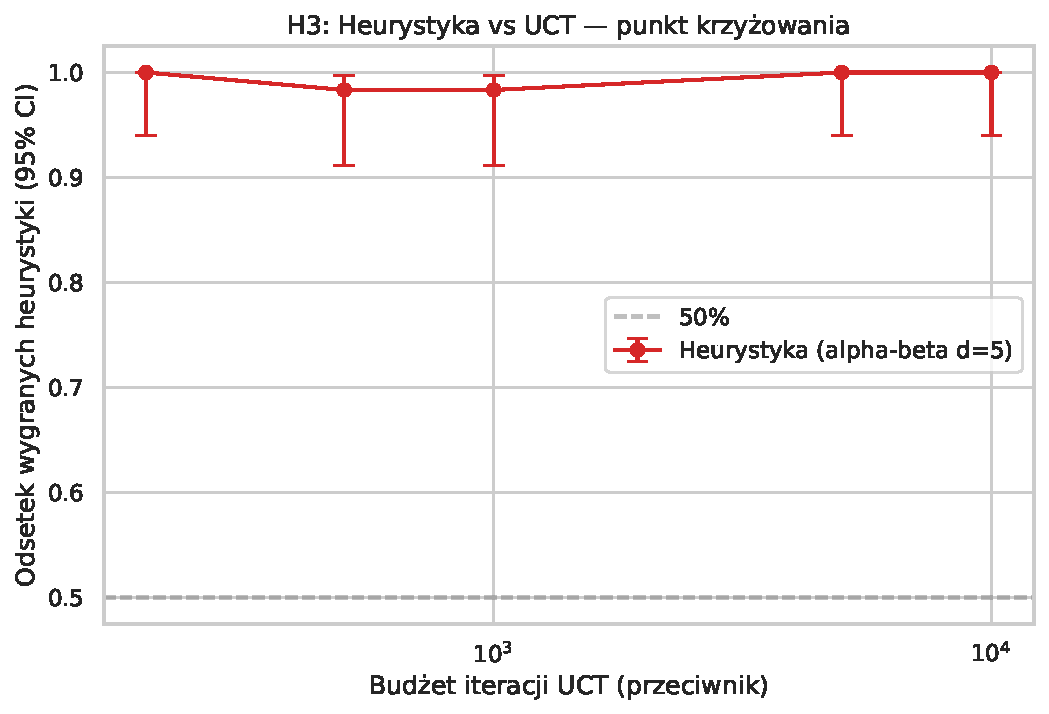
\includegraphics[width=0.85\textwidth]{figures/h3_heuristic_vs_uct}
    \caption{Odsetek wygranych heurystyki (alpha-beta z głębokością 5) względem
    rosnącego budżetu iteracji UCT na planszy 8$\times$8. Oś X logarytmiczna.
    Heurystyka miażdży UCT w całym testowanym zakresie; przy 100\,000 iteracji
    nadal wygrywa 94\% partii --- punkt krzyżowania nie zostaje osiągnięty.}
    \label{fig:h3}
\end{figure}

\paragraph{Dane liczbowe (n=100 partii na budżet, bezpośrednie mecze
heurystyka vs UCT):}

\begin{center}
\begin{tabular}{rcccc}
\toprule
\textbf{Budżet UCT} & \textbf{Heur wygrywa} & \textbf{Win-rate} & \textbf{95\% CI} & \textbf{UCT czas/ruch} \\
\midrule
500      & 99/100  & 99,0\%  & [94,6; 99,8] & $\sim$0,005 s \\
1\,000   & 100/100 & 100,0\% & [96,3; 100]  & $\sim$0,01 s \\
5\,000   & 98/100  & 98,0\%  & [93,0; 99,4] & $\sim$0,05 s \\
10\,000  & 98/100  & 98,0\%  & [93,0; 99,4] & $\sim$0,10 s \\
50\,000  & 94/100  & 94,0\%  & [87,5; 97,2] & $\sim$0,50 s \\
100\,000 & 94/100  & 94,0\%  & [87,5; 97,2] & $\sim$0,97 s \\
\bottomrule
\end{tabular}
\end{center}

Heurystyka pozostaje dominująca w całym praktycznym zakresie. Pierwsza część
hipotezy (wyższość heurystyki przy niskich budżetach) jest spektakularnie
potwierdzona. Druga część (cross-over przy wysokich budżetach) jest
\emph{nieosiągnięta}: win-rate maleje bardzo łagodnie (z 99\% przy UCT(500)
do 94\% przy UCT(100\,000)), pozostając daleko od parytetu. Ekstrapolując ten
trend, teoretyczny cross-over (50\%) leży znacznie powyżej $10^6$ iteracji ---
daleko poza praktycznym zakresem (UCT(100\,000) zajmuje już $\sim$1\,s/ruch).
Na większej planszy 8$\times$8 (głębsze, bardziej taktyczne partie) przewaga
heurystyki jest nawet wyraźniejsza niż przy mniejszych wariantach, ponieważ
losowe symulacje słabiej przybliżają wartość pozycji.

Wynik jest mocnym argumentem za stosowaniem prostych deterministycznych
graczy z funkcją ewaluacji w grach o wyraźnej strukturze taktycznej
i umiarkowanym branching factor. Heurystyka w naszej implementacji wybiera
ruch w $\sim$10 ms (depth 5, 8$\times$8), więc partia $\sim$60 ruchów to
poniżej sekundy --- rzędy wielkości taniej niż UCT(100\,000), a przy tym
istotnie silniej grające.

\subsection{H4: Przewaga pierwszego gracza}
\label{sec:wyniki-h4}

\begin{figure}[ht]
    \centering
    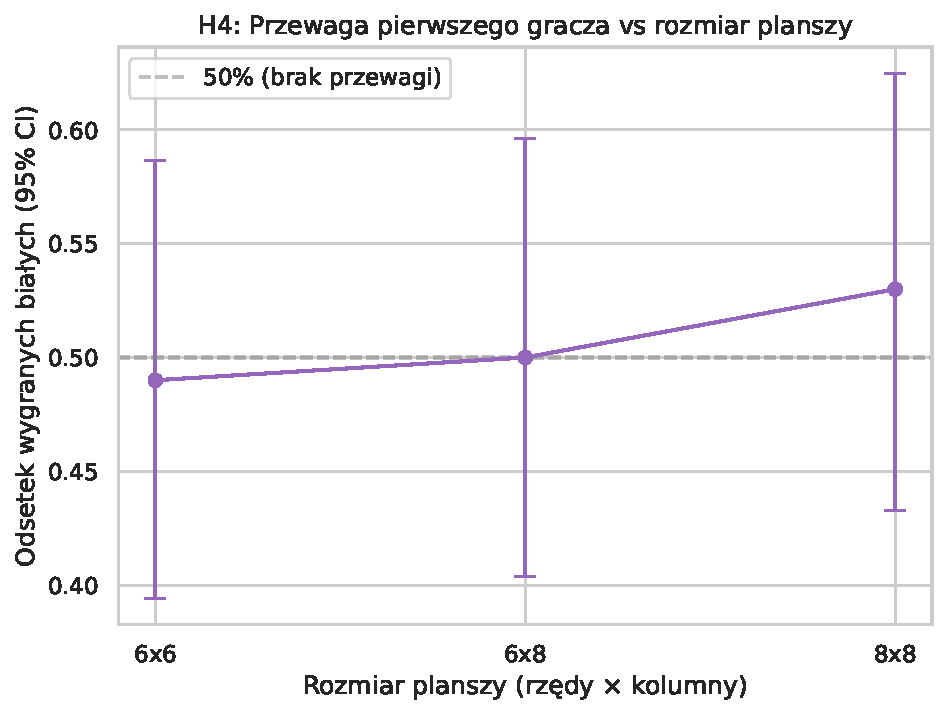
\includegraphics[width=0.5\textwidth]{figures/h4_first_player_advantage}
    \caption{Odsetek wygranych białych (pierwszego gracza) w symetrycznym
    turnieju UCT(5000) vs UCT(5000) na planszy 8$\times$8. Linia 50\% oznacza
    brak przewagi; 95\% CI Wilsona zawiera 50\%.}
    \label{fig:h4}
\end{figure}

\paragraph{Dane liczbowe (n=500 partii):}
Białe wygrały 247/500 = \textbf{49,4\%} partii, 95\% CI Wilsona $[45{,}0\%;\ 53{,}8\%]$
(średnia długość partii ok. 59 ruchów). Przedział obejmuje 50\%, brak więc
istotnej statystycznie przewagi pierwszego gracza.

Hipoteza H4 jest sfalsyfikowana: nie stwierdzamy istotnej statystycznie przewagi
białych. Szerokość CI (ok. $\pm$4,4 pp) jest wystarczająco wąska, by uznać,
że ewentualna ,,prawdziwa'' przewaga jest mniejsza niż 4 pp --- co metodologicznie
odpowiada brakowi przewagi praktycznej.

Interpretacja:
\begin{itemize}[nosep]
    \item Przy MCTS o zbliżonej sile oboje gracze grają sub-optymalnie
          w sposób przybliżonie symetryczny --- przewaga tempa pierwszego
          ruchu zostaje ,,wyzerowana'' przez błędy obu stron.
    \item Możliwe, że przy perfekcyjnej grze (jak w rozwiązanych wariantach
          6$\times$5 \cite{saffidine2011solving} i 6$\times$6
          \cite{bjornsson2026solving}, gdzie wygrywa pierwszy gracz) białe
          rzeczywiście mają przewagę, lecz UCT z 5000 iteracji nie zbliża się
          do tej granicy.
\end{itemize}

\subsection{H5: Strojenie stałej eksploracji $c$}
\label{sec:wyniki-h5}

\begin{figure}[ht]
    \centering
    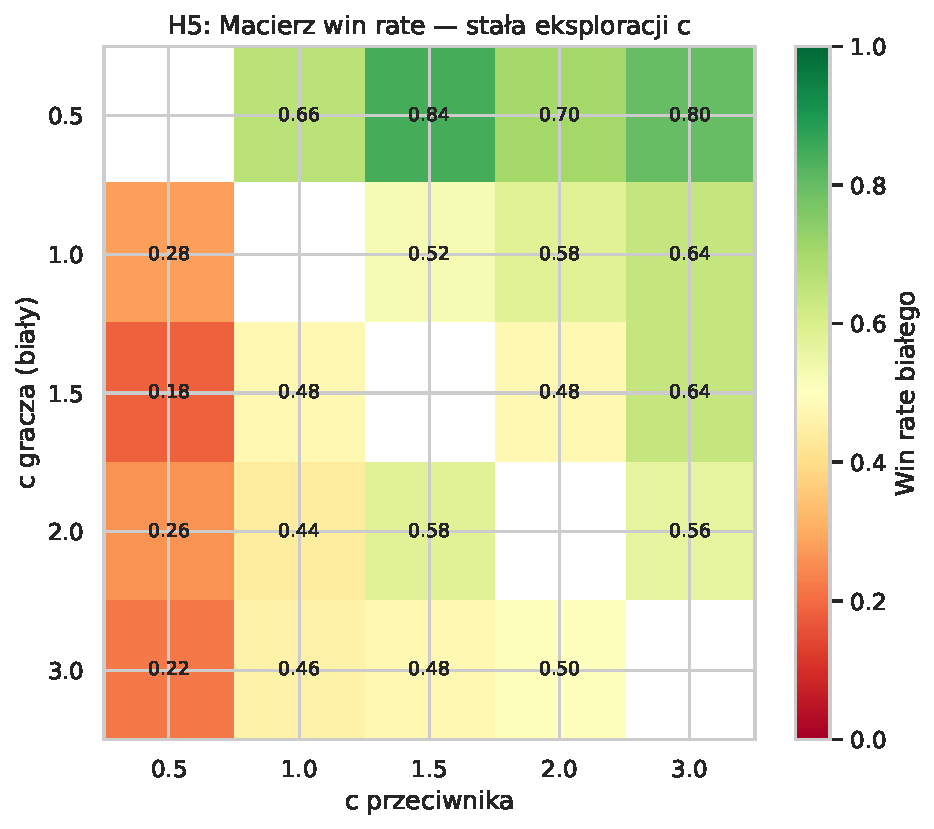
\includegraphics[width=0.7\textwidth]{figures/h5_c_heatmap}
    \caption{Macierz win-rate białych dla turnieju round-robin pięciu wartości
    stałej eksploracji $c$ (UCT 10\,000 iteracji, 8$\times$8). Wiersz --- $c$ gracza
    białego, kolumna --- $c$ przeciwnika. Im niższe $c$ wiersza, tym wyraźniej
    zielony (więcej wygranych): $c = 0{,}5$ dominuje całą tabelę.}
    \label{fig:h5_heatmap}
\end{figure}

\begin{figure}[ht]
    \centering
    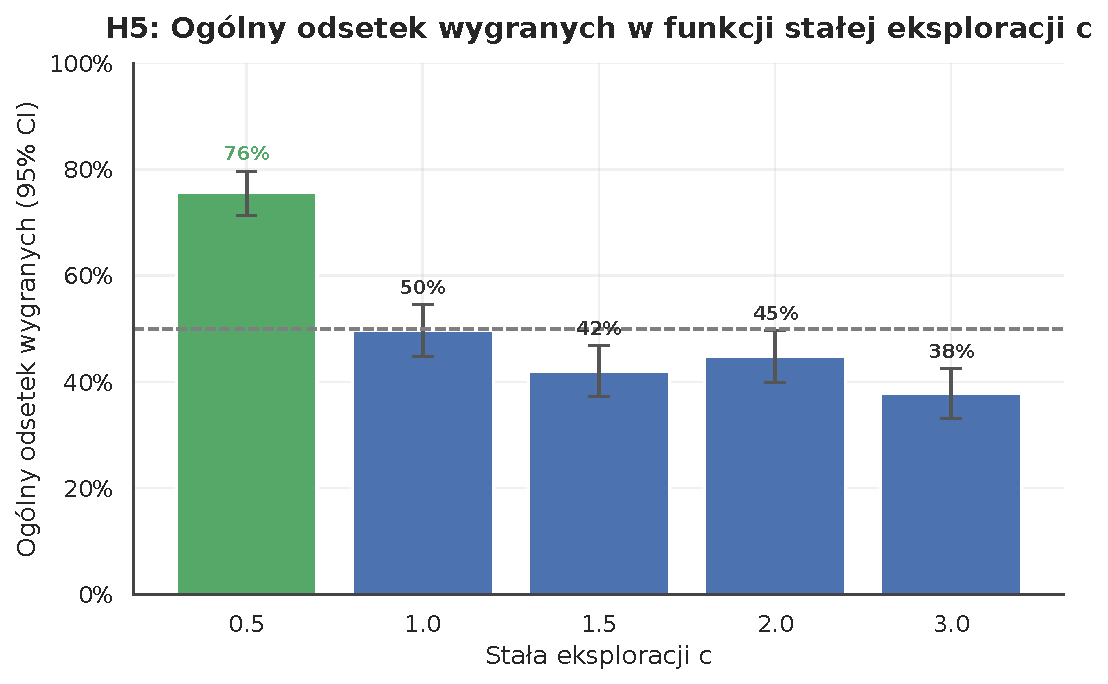
\includegraphics[width=0.7\textwidth]{figures/h5_c_bar}
    \caption{Ogólny win-rate każdej wartości $c$ (uśredniony po obu kolorach
    i wszystkich przeciwnikach). Trend jest w przybliżeniu monotonicznie malejący;
    brak wewnętrznego maksimum w badanym zakresie.}
    \label{fig:h5_bar}
\end{figure}

\paragraph{Dane liczbowe (n=400 partii na wartość $c$):}
\begin{center}
\begin{tabular}{rcccc}
\toprule
\textbf{$c$} & \textbf{Win-rate} & \textbf{95\% CI} & \textbf{$p$ (vs 0,5)} & \textbf{Status} \\
\midrule
0,5 & \textbf{75,7\%} & [71,3; 79,7] & $<10^{-4}$ & najlepsza \\
1,0 & 49,7\% & [44,9; 54,6] & 0,96 & neutralna \\
1,5 & 42,0\% & [37,3; 46,9] & 0,0016 & poniżej 50\% \\
2,0 & 44,8\% & [40,0; 49,6] & 0,040 & poniżej 50\% \\
3,0 & 37,8\% & [33,1; 42,6] & $<10^{-4}$ & najgorsza \\
\bottomrule
\end{tabular}
\end{center}

Hipoteza H5 (istnienie wewnętrznego optimum $c^\star$ o kształcie odwróconego U)
\emph{nie znajduje potwierdzenia} w badanym zakresie. Najsilniejsza okazuje się
\emph{najniższa} testowana wartość $c = 0{,}5$ (75,7\% wygranych, wysoce istotnie),
a win-rate maleje wraz ze wzrostem $c$ --- nie obserwujemy spadku przy małym $c$,
który zamykałby krzywą w kształt odwróconego U. Co więcej, teoretyczna wartość
$c = \sqrt{2} \approx 1{,}41$ (okolice $c = 1{,}5$) wypada wyraźnie poniżej parytetu.

Interpretacja: Breakthrough jest grą silnie taktyczną, w której kluczowe są
konkretne, wymuszone warianty, a nie szerokie zwiedzanie drzewa. Niski $c$
(nacisk na eksploatację) pozwala MCTS głębiej drążyć obiecujące linie, co
przekłada się na realną przewagę. Optymalne $c^\star$ leży zatem \emph{na lub
poniżej} dolnej granicy testowanego zakresu --- co stanowi praktyczną wskazówkę
do strojenia UCT w tej grze i sugeruje rozszerzenie eksperymentu o $c \in \{0{,}1,\ 0{,}25\}$.

\subsection{H6: Czas decyzji w funkcji numeru ruchu}
\label{sec:wyniki-h6}

\begin{figure}[ht]
    \centering
    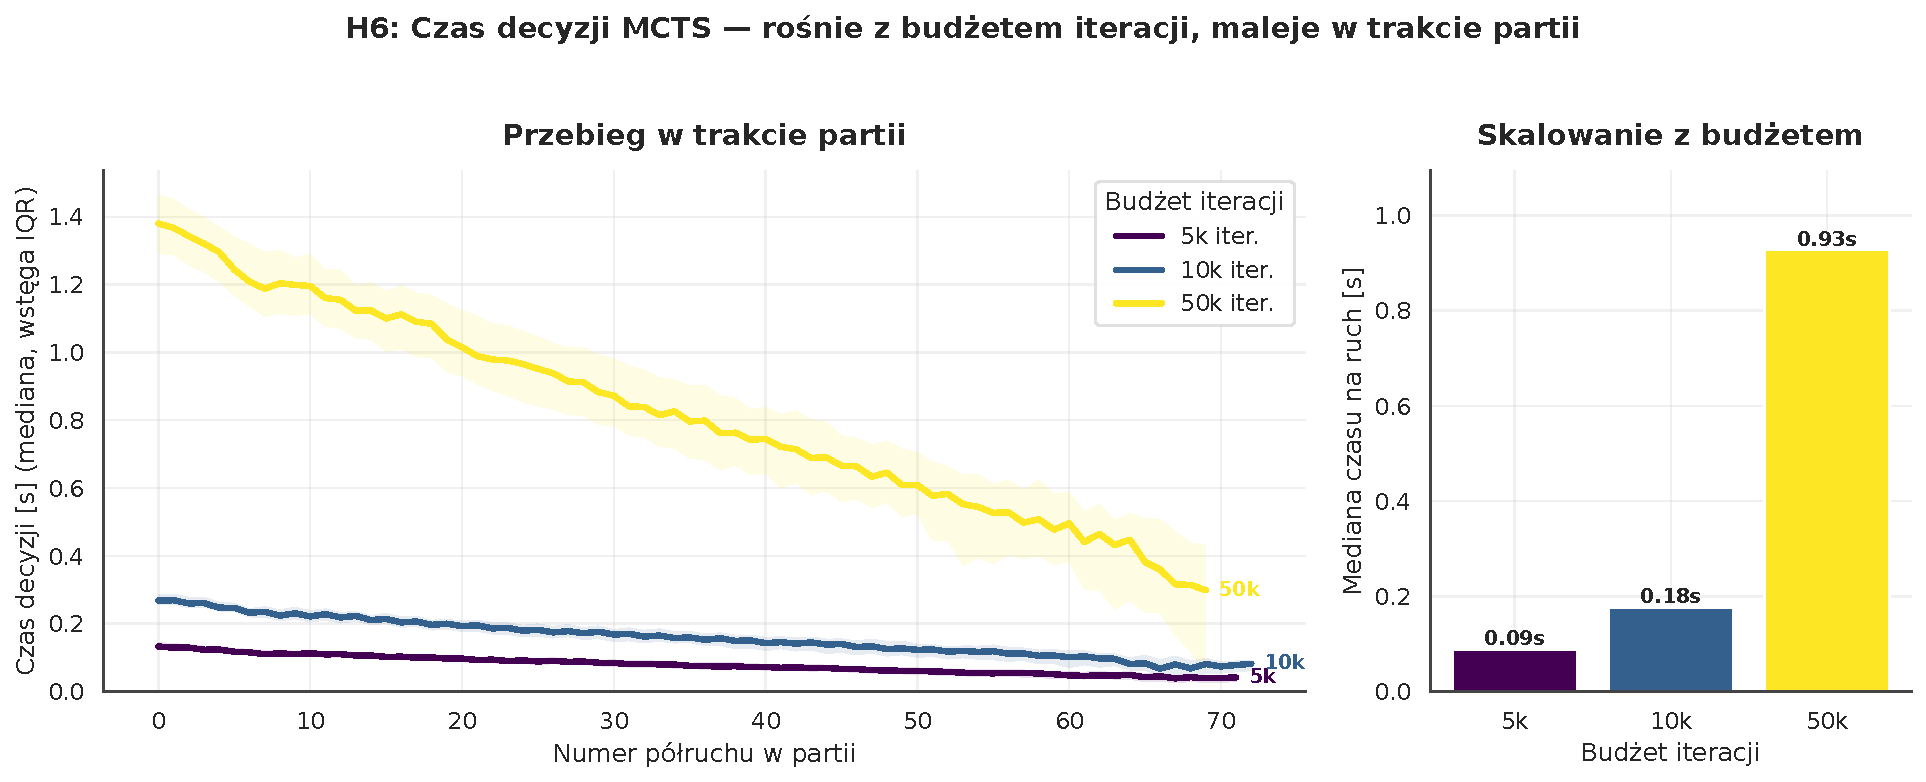
\includegraphics[width=0.95\textwidth]{figures/h6_decision_time}
    \caption{Średni czas decyzji UCT w funkcji numeru ruchu, w rozbiciu na budżet
    iteracji (8$\times$8). Czas jest najwyższy w otwarciu i maleje monotonicznie
    w trakcie partii. Charakterystyczny ząbkowany kształt wynika z naprzemiennej
    gry agentów o różnych budżetach (kolejne ruchy wykonują różni gracze).}
    \label{fig:h6}
\end{figure}

\paragraph{Średni czas decyzji wg budżetu iteracji:}
\begin{center}
\begin{tabular}{rcc}
\toprule
\textbf{Budżet UCT} & \textbf{Średni czas/ruch} & \textbf{Odch.\ std.} \\
\midrule
5\,000   & 0,298 s & 0,364 s \\
10\,000  & 0,354 s & 0,389 s \\
50\,000  & 0,517 s & 0,453 s \\
\bottomrule
\end{tabular}
\end{center}

Hipoteza H6 (czas decyzji rośnie w środkowej fazie gry) jest \emph{sfalsyfikowana}.
Wbrew oczekiwaniom, średni czas na ruch jest \emph{najwyższy w otwarciu}
i maleje monotonicznie w miarę postępu partii --- nie obserwujemy maksimum
w ruchach 15--40. Wyjaśnienie tkwi w naturze kosztu pojedynczej iteracji MCTS:
przy stałym budżecie iteracji dominującym kosztem jest długość losowej symulacji
(rolloutu do stanu terminalnego), a ta jest najdłuższa na początku gry i kurczy
się wraz ze zbliżaniem do końcówki. Większy branching factor w środkowej fazie
\emph{nie} podnosi kosztu ruchu, ponieważ liczba iteracji jest ustalona.
Zgodnie z oczekiwaniem skaluje się natomiast czas z budżetem (0,30 s $\to$
0,52 s dla 5k $\to$ 50k iteracji).

\subsection{Synteza ilościowa}

Tabela~\ref{tab:synteza} podsumowuje status każdej hipotezy.

\begin{table}[ht]
\centering
\caption{Synteza wyników eksperymentalnych.}
\label{tab:synteza}
\begin{tabular}{p{3cm}p{6cm}p{4cm}}
\toprule
\textbf{Hipoteza} & \textbf{Wynik} & \textbf{Status} \\
\midrule
H1: RAVE > UCT &
49,0 / 48,0 / 54,0 / 39,0\%
(@ 5k / 10k / 50k / 100k iter) &
Sfalsyfikowana \\
\midrule
H2: PB > UCT &
50,0 / 43,0 / 55,0 / 46,0\%
(@ 5k / 10k / 50k / 100k iter) &
Niejednoznaczna \\
\midrule
H3: heurystyka > UCT przy niskim budżecie, < UCT przy wysokim &
99\% $\to$ 94\%
(@ 500--100\,000 iter) &
Częściowo potwierdzona \\
\midrule
H4: białe mają przewagę &
49,4\% wygranych białych
(8$\times$8, n=500) &
Sfalsyfikowana \\
\midrule
H5: $c$ ma nieliniowy wpływ (optimum $c^\star$) &
najlepsze $c=0{,}5$ (75,7\%), monotoniczny spadek do $c=3{,}0$ (37,8\%) &
Sfalsyfikowana \\
\midrule
H6: czas decyzji rośnie w środku gry &
czas maleje monotonicznie od otwarcia &
Sfalsyfikowana \\
\bottomrule
\end{tabular}
\end{table}

\section{Wnioski}
\label{sec:wnioski}

\subsection{Synteza i kluczowe odkrycie}

Najbardziej zaskakującym wynikiem projektu jest \textbf{nieskuteczność
RAVE w Breakthrough 8$\times$8}. Pokazuje to, że standardowe techniki rozwoju
MCTS są domain-specific: założenie ,,dobrego ruchu zagranego gdziekolwiek''
(kluczowe dla AMAF) działa świetnie w Go, lecz załamuje się w grze, gdzie
te same fizyczne ruchy mają radykalnie różną wartość w zależności od pozycji.
Co istotne, wynik ten nie jest artefaktem implementacji -- poprawność szkieletu
RAVE potwierdziliśmy testem $\beta \to 0$ (odtworzenie siły UCT), więc spadek
pochodzi z samej heurystyki AMAF.

Drugim ważnym wnioskiem jest \textbf{przygniatająca przewaga prostej heurystyki
alpha-beta} dla tej klasy gier. Heurystyka oparta na bogatej funkcji ewaluacji
(wykładnicze zaawansowanie, groźba przebicia, obrońcy, centralność, swobodna
ścieżka, izolacja, mobilność i materiał -- Algorytm~1) z głębokością 5 i
porządkowaniem ruchów dominuje MCTS w całym praktycznym zakresie iteracji
(94\% nawet przy 100\,000 iteracji UCT), grając przy tym rzędy wielkości szybciej.

Trzecim, praktycznym odkryciem jest \textbf{korzyść z niskiej stałej eksploracji}
(H5): w taktycznym Breakthrough $c = 0{,}5$ wyraźnie przewyższa kanoniczne
$c = \sqrt{2}$, co sugeruje, że gra premiuje eksploatację (głębsze drążenie
wymuszonych wariantów) nad eksploracją.

\subsection{Propozycje dalszych prac}

\begin{itemize}[nosep]
    \item \textbf{Polityka rolloutowa oparta na heurystyce.} Jednym z najprostszych
          rozszerzeń byłaby zamiana czysto losowych symulacji na epsilon-greedy
          po heurystyce (np. ulubione ruchy z funkcji ewaluacji). Powinno to
          drastycznie poprawić wszystkich agentów MCTS i może zmienić
          rezultat H1 (RAVE z heurystycznymi rolloutami).
    \item \textbf{MAST i NAST.} Alternatywne techniki uczące się polityki
          symulacyjnej -- Move-Average Sampling Technique \cite{finnsson2008simulation}
          -- mogłyby przewyższyć heurystykę w niskim/średnim zakresie
          iteracji. To naturalna kontynuacja H2.
    \item \textbf{Krzyżowanie z deep RL.} Implementacja prostej sieci ewaluacyjnej
          (jak w AlphaZero, lecz z mniejszą architekturą) i jej porównanie
          z heurystyką alpha-beta.
\end{itemize}

\section{Użycie LLM w projekcie}

% TODO: Wymagane przez prowadzącego. Pokryj szczegółowo:
%  1. Lista zadań delegowanych do Claude Opus 4.7 (np. szkielet repo, silnik gry,
%     warianty MCTS, harness eksperymentów, GUI, skrypty analityczne, raport)
%  2. Każdy fragment podlegał review autorów --- udokumentowane w commitach git
%  3. Bugi wykryte w wygenerowanym kodzie i sposób ich naprawy (np. issue z
%     wraparoundem przesunięć, validacja from_string, overflow w u8 multiplication)
%  4. Użycie LLM do raportu: pomoc w strukturze, formułowaniu, ale wszystkie
%     interpretacje wyników i twierdzenia merytoryczne pochodzą od autorów
%  5. Świadomość ograniczeń: weryfikacja statystyczna nadal po stronie autorów

\subsection{Zakres użycia}
[Co dokładnie zostało wygenerowane przez LLM, co napisali autorzy.]

\subsection{Proces weryfikacji}
[Kod review, testy cross-validation, code review LLM]

\subsection{Wykryte błędy}
[Lista bugów wykrytych w wygenerowanym kodzie i jak je naprawiono.]

\subsection{Świadomość ograniczeń}
[Zasady używania LLM, ostatnia decyzja zawsze należy do autorów.]


\printbibliography

\end{document}
